%% ma: L12-B13-0018
%% lop: 12
%% chuong: 4
%% bai: 13
%% dang: 12.13.10
%% loai: DS
%% muc: [TH, TH, VD, VDC]
%% dap_an: "SSĐĐ"
%% nguon: "(NBV)-ĐỀ SỐ 6-MỖI NGÀY 1 ĐỀ THI 2025.pdf (D06, MỖI NGÀY 1 ĐỀ - Đề số 6), Phần II Câu 4 (theo Howard Anton, Irl C. Bivens, Calculus AP Edition 11E)"
%% kien_thuc: "Bài 13 (ứng dụng tích phân: thể tích vật thể qua diện tích thiết diện S(x); công); Bài 27 lớp 11 (thể tích khối nón, khối trụ)"
%% trang_thai: chinh-thuc
%% ghi_chu: "Giáo viên duyệt gợi ý sửa 10/10/2026. Đề gốc mâu thuẫn (bể trụ cao 0,75 m ứng với thể tích 12π nhưng lời giải gốc dùng lớp chất lỏng x từ 5 đến 9 có thể tích 604π/27); đã sửa: chất lỏng trong bể nón cao 4 m tính từ đáy (x từ 5 đến 9), bể trụ cao khoảng 1,4 m. Đáp án giữ nguyên S S Đ Đ (kiểm bằng sympy: W=518013,7≈518014 Jun). Hình dựng lại theo hình gốc (đỉnh nón O ở trên, trục x hướng xuống)"
\begin{ex}
Một bể hình nón có bán kính đáy là $3$ m và chiều cao là $9$ m đang chứa một lượng chất lỏng. Công thức tính công để hút toàn bộ lượng nước này ra khỏi bể là $W=\displaystyle\int_a^b\rho xS(x)\,\mathrm dx$ (Jun) trong đó $\rho$ $(\text{kg}/\text{m}^3)$ là khối lượng riêng của chất lỏng, $S(x)$ là diện tích mặt cắt (theo Howard Anton, Irl C. Bivens, Calculus AP Edition, 11E, 2016, Wiley).
\begin{center}
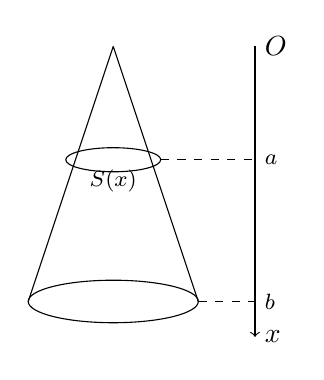
\begin{tikzpicture}[scale=.9]
  \draw (0,3.6)--(-1.2,0) (0,3.6)--(1.2,0);
  \draw (0,0) ellipse (1.2 and .3);
  \draw (0,2) ellipse (.67 and .17);
  \draw[dashed] (.67,2)--(2,2) (1.2,0)--(2,0);
  \draw[->] (2,3.6)--(2,-.5) node[right]{$x$};
  \path (2,3.6) node[right]{$O$} (2,2) node[right,font=\footnotesize]{$a$} (2,0) node[right,font=\footnotesize]{$b$};
  \path (0,2) node[below,font=\footnotesize]{$S(x)$};
\end{tikzpicture}
\end{center}
Biết chất lỏng trong bể hình nón có độ cao $4$ m tính từ đáy bể. Từ bể này, người ta hút hết lượng chất lỏng và bơm sang một bể hình trụ có bán kính đáy là $4$ m, khi đó thấy lượng chất lỏng trong bể hình trụ cao khoảng $1{,}4$ m.
\choiceTF
{Thể tích chất lỏng là $27\pi$ $(\text{m}^3)$.}
{Chiều cao lượng chất lỏng khi chứa trong bể hình nón là $9$ m.}
{\True Diện tích mặt cắt $S(x)=\dfrac{\pi x^2}{9}$.}
{\True Biết khối lượng riêng của chất lỏng này là $1000\ \text{kg}/\text{m}^3$. Khi đó, công để hút nước từ bể hình nón sang bể hình trụ là $W=518014$ (Jun) (kết quả được làm tròn đến hàng đơn vị của Jun).}
\loigiai{Chất lỏng chiếm lớp từ $x=5$ đến $x=9$ (cao $4$ m tính từ đáy). Với $O$ là đỉnh nón, tiết diện ở độ sâu $x$ có bán kính $\dfrac x3$ nên $S(x)=\dfrac{\pi x^2}9$: c) đúng.

a) Thể tích chất lỏng là $\displaystyle\int_5^9\dfrac{\pi x^2}9\,\mathrm dx=\dfrac{604\pi}{27}\approx22{,}4\pi\ \text{m}^3$ (khớp với $\pi\cdot4^2\cdot1{,}4\approx22{,}4\pi$), còn $27\pi$ là thể tích cả bể nón. Sai.

b) Chiều cao lớp chất lỏng là $4$ m, không phải $9$ m. Sai.

d) $W=\displaystyle\int_5^9 1000\cdot\dfrac{\pi x^3}9\,\mathrm dx=\dfrac{1000\pi}{36}\left(9^4-5^4\right)\approx518\,014$ Jun. Đúng.}
\end{ex}
